\chapter{Design}




\section{Component diagram}

The system will be organized in a classical client-server configuration, and the latter will expose RESTful APIs to the clients, and a web application for both OPs and PRs. Every service will be in its own servlet. The component diagram is shown in Figure \ref{fig:component}.

\begin{figure}[h]
    \centering
    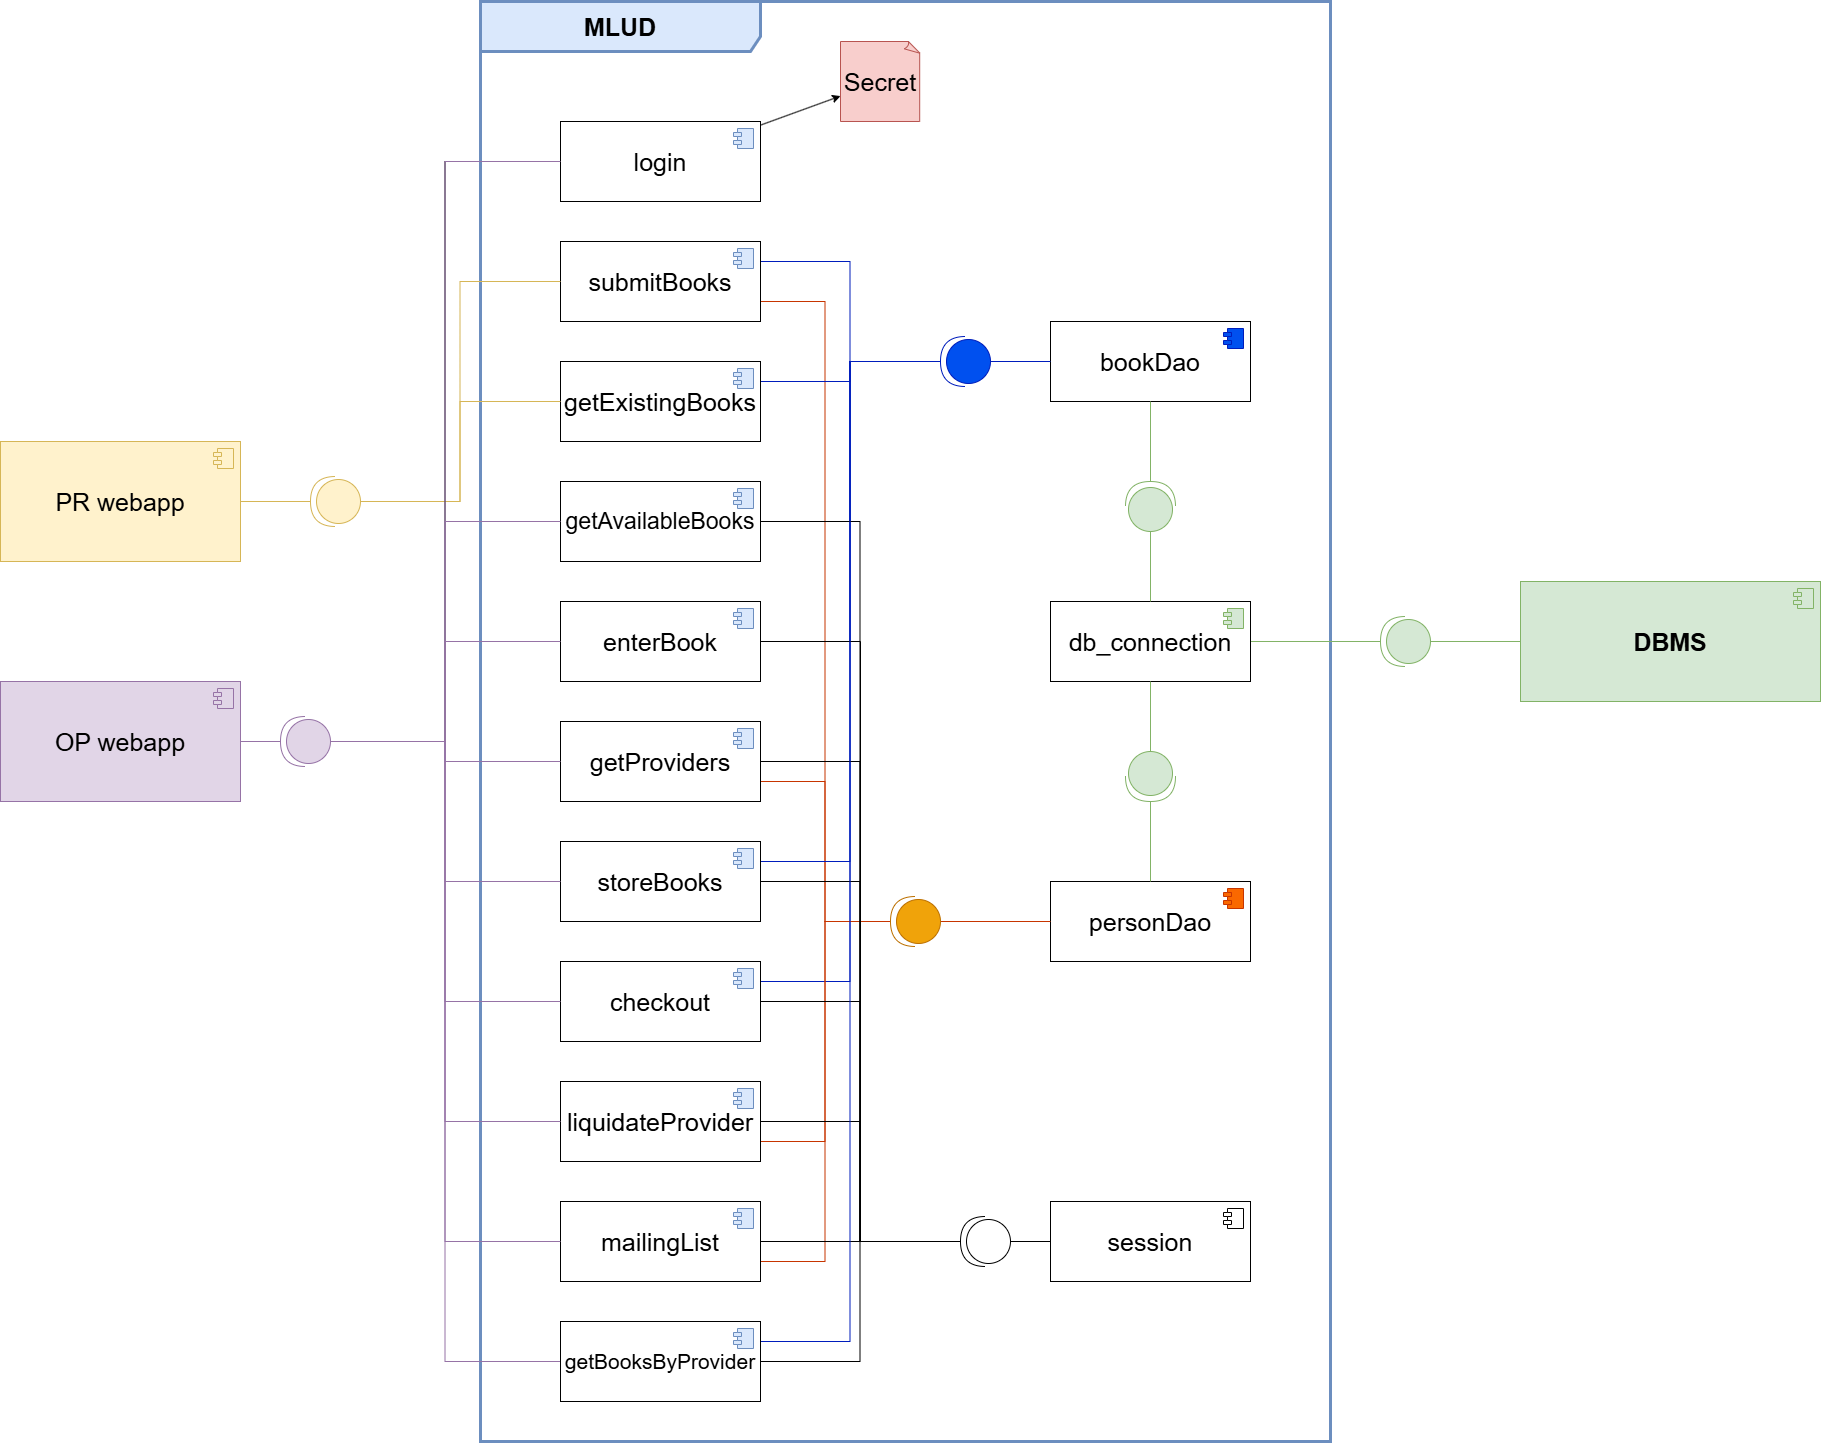
\includegraphics[width=\textwidth]{assets/component_diagram.png}
    \caption{Component diagram}
    \label{fig:component}
\end{figure}

\section{Logical description of data}

The data will be stored into a relational database, which will be designed according to the Logical schema in Figure \ref{fig:er}.

\begin{figure}[h]
    \centering
    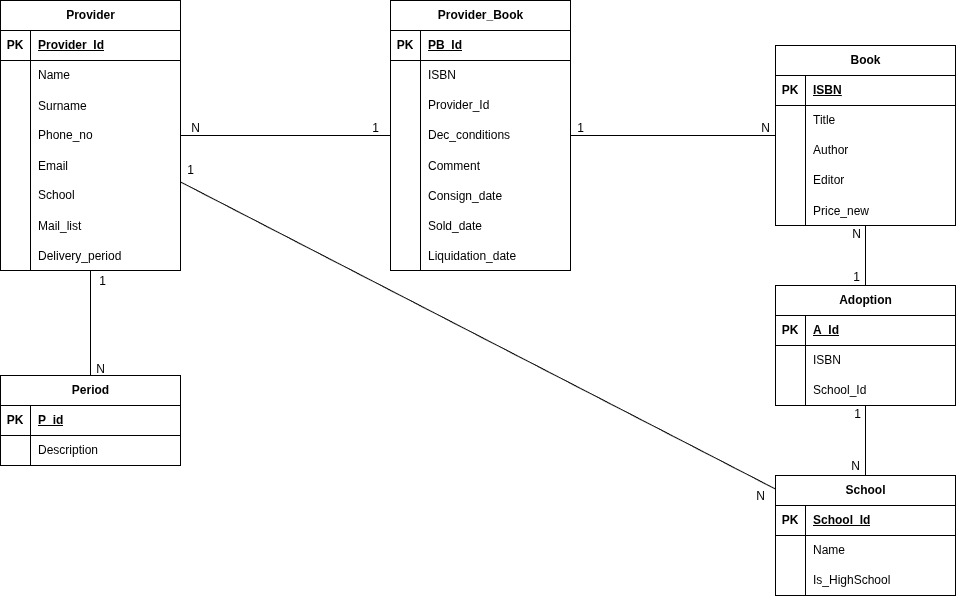
\includegraphics[width=\textwidth]{assets/er_diagram.png}
    \caption{Logical schema of the database}
    \label{fig:er}
\end{figure}

\section{API endpoints}

The API will expose the endpoints in a structure coherent with the compoenent diagram \ref{fig:component}. It follows a list of the endpoints:

\subsection{Login}
\textbf{Method} : POST \\
\textbf{EndPoint} : /login.php \\
\textbf{Body parameters} :
\begin{lstlisting}[language=JavaScript, label={lst:jscode}, basicstyle=\ttfamily]
{ "Hashed_password": String }
\end{lstlisting}
\textbf{Response} : \texttt{200} if the login is successful, \texttt{401} if the password is wrong.

\subsection{Submit Books}
A PR submits its books to the system, and gives its personal information.\\
\textbf{Method} : POST \\
\textbf{EndPoint} : /submitBooks.php \\
\textbf{Body parameters} :
\begin{lstlisting}[language=JavaScript, label={lst:jscode}, basicstyle=\ttfamily]
{
    "Name": String,
    "Surname": String,
    "School": String,
    "Email": String,
    "Phone": String,
    "Books": [
        {
            "ISBN": String,
            "Title": String,
            "Author": String,
            "Editor": String,
            "Price_new": Number,
            "Dec_conditions": String
        },
        ...
    ],
    "Mail_list": Boolean // TODO: actually add it into the database and the form
}
\end{lstlisting}
\textbf{Response} : \texttt{200} if the submission is successful, \texttt{400} if the request is malformed.

\subsection{Get Existing Books}
The system returns the information of the books already in the system, searching by ISBN.\\
\textbf{Method} : GET \\
\textbf{EndPoint} : /getExistingBooks.php \\
\textbf{URL parameters} :
\begin{itemize}
    \item \texttt{ISBN}: String
\end{itemize}
\textbf{Response} :
\begin{lstlisting}[language=JavaScript, label={lst:jscode}, basicstyle=\ttfamily]
[
    {
        "ISBN": String,
        "Title": String,
        "Author": String,
        "Editor": String,
        "Price_new": Number
    },
    ...
]
\end{lstlisting}

\subsection{Get Books in Stock}
The system returns all the books in stock, i.e. the books both submitted and actually delivered by the PRs.\\
\textbf{Method} : GET \\
\textbf{EndPoint} : /getAvailableBooks.php \\
\textbf{Response} :
\begin{lstlisting}[language=JavaScript, label={lst:jscode}, basicstyle=\ttfamily]
[
    {
        "ISBN": String,
        "Title": String,
        "Author": String,
        "Editor": String,
        "Price_new": Number,
        "ProviderName": String,
        "ProviderSurname": String,
        "PB_Id": Number,
        "Provider_Id": Number,
        "Dec_conditions": String,
        "Comments"? : String,
        "Consign_date": String,
        % // didn't have the sbatta to remove them from the select
        "Sold_date": null, 
        "Liquidation_date": null

    },
    ...
]
\end{lstlisting}

\subsection{Enter book}
An OP enters a book in the system, associating it to a ISBN. No strong need for this, it's just to make simpler the PR submission.\\
\textbf{Method} : POST \\
\textbf{EndPoint} : /enterBook.php \\
\textbf{Body parameters} :
\begin{lstlisting}[language=JavaScript, label={lst:jscode}, basicstyle=\ttfamily]
{
    "ISBN": String,
    "Title": String,
    "Author": String,
    "Editor": String,
    "Price_new": Number
}
\end{lstlisting}
\textbf{Response} : \texttt{200} if the submission is successful, \texttt{400} if the request is malformed.

\subsection{Get PRs}
The system returns the list of PRs, to handle the delivery of the books and the liquidation.
\textbf{Method} : GET \\
\textbf{EndPoint} : /getProviders.php \\
\textbf{Response} :
\begin{lstlisting}[language=JavaScript, label={lst:jscode}, basicstyle=\ttfamily]
[
    {
        "ISBN": String,
        "Title": String,
        "Author": String,
        "Editor": String,
        "Price_new": Number,
        "Name": String,
        "Surname": String,
        "PB_Id": Number,
        "Provider_Id": Number,
        "Dec_conditions": String,
        "Comments"? : String,
        "Consign_date"?: String,
        "Sold_date"?: String,
        "Liquidation_date"?: String,
        "Phone_no": String,
        "Email": String,
        "School": String
    },
    ...
]
\end{lstlisting}

\subsection{Deliver Books}
A PR delivers the books to the OP.\\
\textbf{Method} : POST \\
\textbf{EndPoint} : /storeBooks.php \\
\textbf{Body parameters} :
\begin{lstlisting}[language=JavaScript, label={lst:jscode}, basicstyle=\ttfamily]
[
    {
        "PB_Id": Number,
        "Comments"?: String
    },
    ...
]
\end{lstlisting}
\textbf{Response} : \texttt{200} if the submission is successful, \texttt{400} if the request is malformed.

\subsection{Sell Books}
An OP sells the books to a BY.\\
\textbf{Method} : POST \\
\textbf{EndPoint} : /sellBooks.php \\
\textbf{Body parameters} :
\begin{lstlisting}[language=JavaScript, label={lst:jscode}, basicstyle=\ttfamily]
[
    { "PB_Id": Number },
    ...
]
\end{lstlisting}
\textbf{Response} : \texttt{200} if the submission is successful, \texttt{400} if the request is malformed.

\subsection{Liquidate PR and return unsold books}
An OP liquidates the PR, returning the unsold books and the money.\\
\textbf{Method} : POST \\
\textbf{EndPoint} : /liquidateProvider.php \\
\textbf{Body parameters} :
\begin{lstlisting}[language=JavaScript, label={lst:jscode}, basicstyle=\ttfamily]
{ "Provider_Id": Number, }
\end{lstlisting}
\textbf{Response} : \texttt{200} if the submission is successful, \texttt{400} if the request is malformed.

\subsection{Mailing list}
Show the list of PRs that accepted to be in the mailing list.\\
\textbf{Method} : GET \\
\textbf{EndPoint} : /mailingList.php \\
\textbf{Response} :
\begin{lstlisting}[language=JavaScript, label={lst:jscode}, basicstyle=\ttfamily]
[
    {
        "Name": String,
        "Surname": String,
        "Email": String
    },
    ...
]
\end{lstlisting}


\section{Deployment}

All the webapp will be entirely deployed on the free hosting service \href{www.altervista.org}{Altervista}, which provides a MySQL database and a php server, so all the problems of deployment, reliability, scalability, and security are handled by the service provider.

\section{UX design}

The webapp will be designed with a simple and intuitive interface, with a clean and modern look. 

The UX is explained at an high level in the flow diagrams in Figures \ref{fig:flow_book_submission} and \ref{fig:flow_op}.

\begin{figure}[ht]
    \centering
    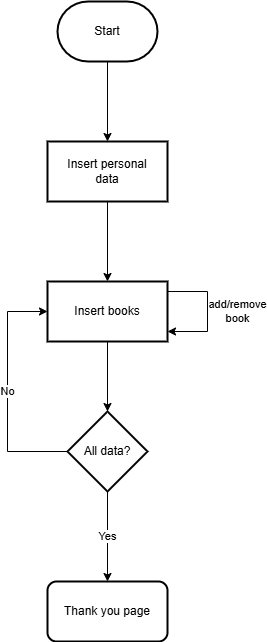
\includegraphics[width=.25\textwidth]{assets/flow_book_submission.png}
    \caption{Flow of the book submission}
    \label{fig:flow_book_submission}
\end{figure}

\begin{figure}[ht]
    \centering
    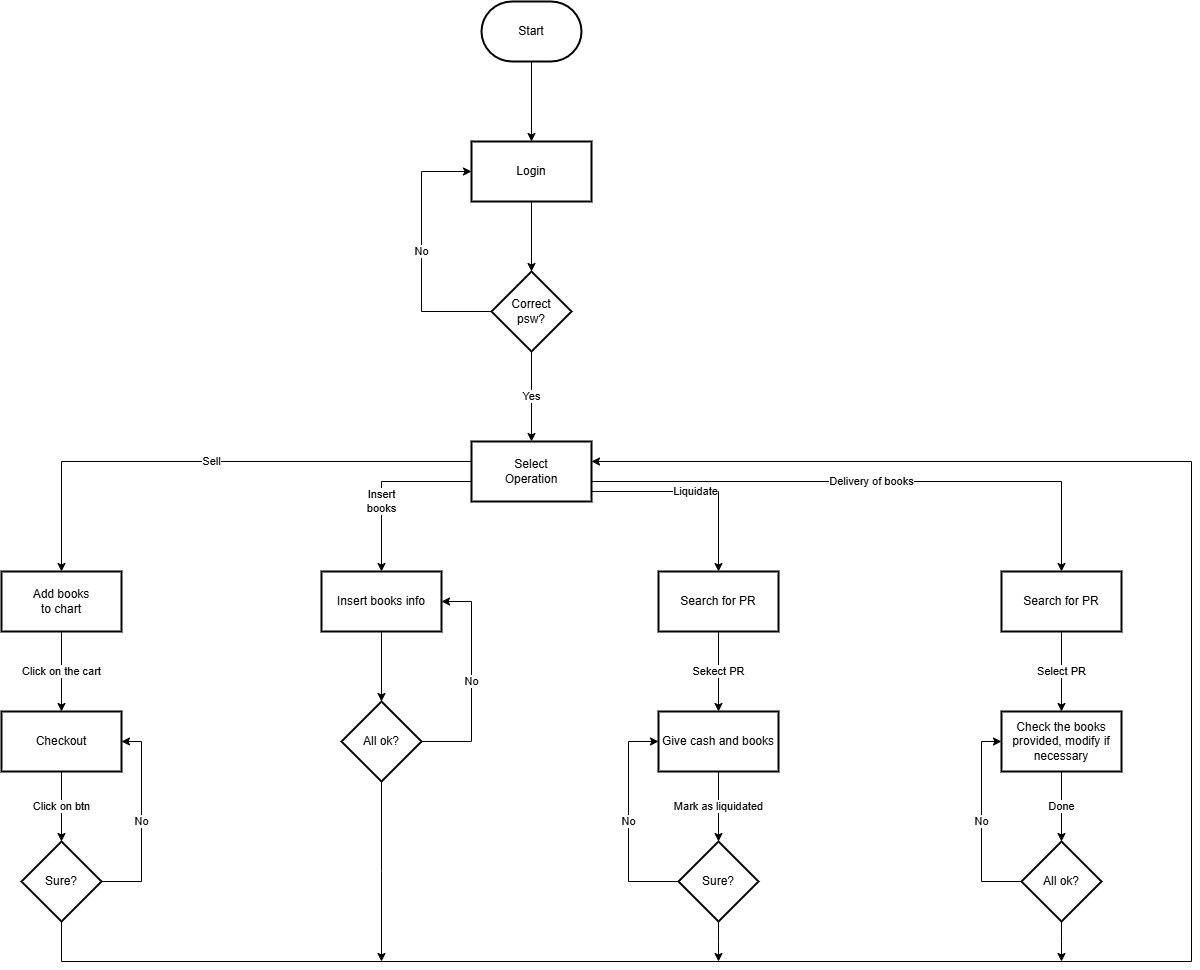
\includegraphics[width=\textwidth]{assets/flow_op.png}
    \caption{Flow of the OP}
    \label{fig:flow_op}
\end{figure}

\section{User interface}

Still WIP. Screenshots will be added in a future release of the document.